\chapter{Experimentación}

En este capítulo se recoge el desarrollo de los experimentos llevados a cabo en este trabajo y todos los resultados que se han obtenido empíricamente de estos.

\section{Bibliotecas y desarrollo de los experimentos}

Para el desarrollo de los experimentos usaremos las bibliotecas de aprendizaje profundo \textbf{PyTorch} para la construcción de la estructura del proyecto y \textbf{Fastai} biblioteca extensión de PyTorch para el proceso de entrenamiento de los modelos. Construiremos nuestras propias clases en PyTorch para la construcción de las arquitectura y para la creación de la instancia de trabajo de nuestro dataset. Tenemos las siguientes componentes.

\begin{enumerate}
	\item \textbf{Clase del Dataset: BraTS}. Clase que representa al conjunto de datos. Sus funciones principales son \texttt{len(self)} que devuelve la cantidad de datos en la clase y \texttt{getitem(self, index)} que devuelve un dato de la clase dado un índice. Esta clase hereda de la clase \textbf{Dataset} de PyTorch.
	La instancia de esta clase será la entrada a la clase \textbf{DataLoader} de PyTorch.
	
	\item \textbf{Clases de las arquitecturas: SegNet y BinaryNet}. Implementan las arquitecturas para clasificación y segmentación. Aparte del constructor que es donde se define la arquitectura tiene la función \texttt{forward(self, x)} que define como se infiere por la red. PyTorch solo necesita la definición de la inferencia para calcular automáticamente la función \texttt{backward} internamente la función para la aplicación de backpropagation (necesario en el entrenamiento). Usa las instancias de los módulos siguientes.
	
	\item \textbf{Clases de los módulos de subida y bajada: DownConv y UpConv}. Análogas a las clases de la arquitecturas pero reduciéndolo a una parte. Usa la instancia de la clase siguiente (ya que sólo definimos uno de estos bloques por módulo).
	
	\item \textbf{Clase de un bloque de convolución: ConvBlock}. Clase que define las capas de un bloque de en nuestra red. Dentro del constructor llama a las funciones de PyTorch de ReLU, convolución y batch normalization.
	
\end{enumerate}

A continuación, podemos ver en detalle la estructura de todos nuestros experimentos a través de un diagrama de clases.

\begin{figure}[H]
	\centering
	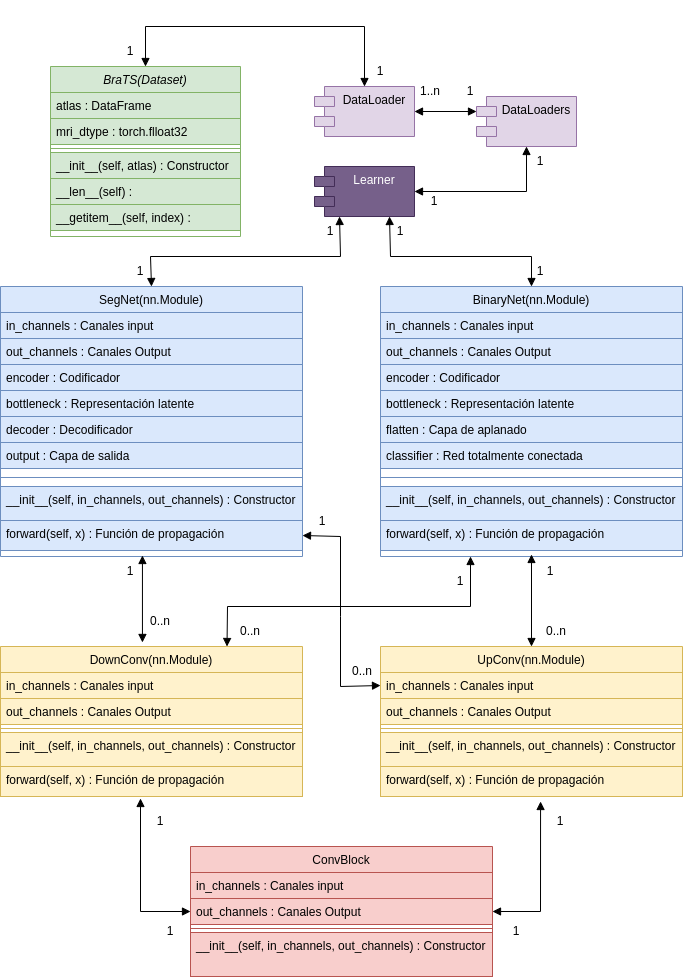
\includegraphics[width=0.75\linewidth]{imagenes/clases_pytorch.png}
	\caption{Diagrama de clases de PyTorch}
\end{figure}

\section{Construcción del codificador y representación latente}

Pasamos a comentar los experimentos llevados cabo en la tarea de la reconstrucción de imágenes.

\subsection{Arquitecturas con conexiones residuales: ResNet34}

Comenzamos ajustando \textbf{ResNet34} a las imágenes. Tras $7$ épocas sumando un total de $8$ horas $30$ minutos de entrenamiento para toda la red obtenemos estos resultados.
Podemos ver los resultados en forma tabular y en forma de gráfica. En la gráfica el eje $Y$ representa la pérdida y el eje $X$ representa la cantidad de imágenes vistas (aunque haya visto la misma imagen más de una vez en distintas épocas). 

\begin{table}[H]
	\centering
	\begin{tabular}{|ccccc|}
		\toprule
		epoch & train\_loss & valid\_loss & MAE & time \\ 
		\midrule
		0 & 0.098790 & 0.111301 & 0.111301 & 1:09:46 \\ 
		0 & 0.079261 & 0.081548 & 0.081548 & 1:13:33 \\
		2 & 0.071293 & 0.075421 & 0.075421 & 1:14:20 \\ 
		3 & 0.064748 & 0.067580 & 0.067580 & 1:14:41 \\ 
		4 & 0.059911 & 0.062933 & 0.062933 & 1:15:55 \\ 
		5 & 0.057501 & 0.059307 & 0.059307 & 1:15:36 \\ 
		6 & 0.055986 & 0.058405 & 0.058405 & 1:15:37 \\ 
		\bottomrule
	\end{tabular}
	\caption{Pérdida de entrenamiento y validación para la reconstrucción con ResNet34}
	\label{tabla:resultados2}
\end{table}

\begin{figure}[H]
	\centering
	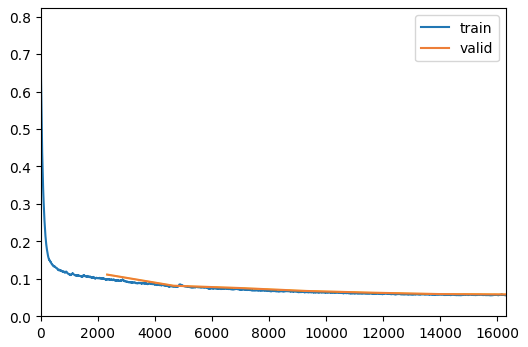
\includegraphics[width=0.7\linewidth]{imagenes/curva_resnet34.png}
	\caption{Curva de aprendizaje con ResNet34}
\end{figure}

Observamos una rápida convergencia la inicio y un entrenamiento perfecto con ambos errores muy cercanos en todas las épocas $E_{val} \approx E_{train}$. Indicando que el proceso de entrenamiento está realizando correctamente y que la arquitectura es válida para aprender a reconstruir las imágenes. Finalmente, obtenemos un $E_{val} \approx 0.058$ lo cual indica que nuestra red reconstruye las imágenes con una pérdida del $5.8 \%$ de los detalles reales.

A continuación, observamos cómo la red reconstruye tres imágenes. En la siguiente salida vemos tres imágenes donde podemos apreciar la salida de la red como la imagen de la izquierda de cada pareja y la imagen real a la derecha.

\begin{figure}[H]
	\centering
	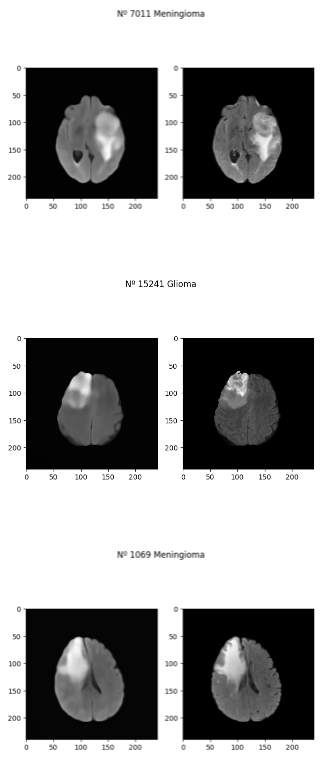
\includegraphics[width=0.4\linewidth]{imagenes/reconstruccion_resnet34.png}
	\caption{Reconstrucción de las imágenes con ResNet34}
\end{figure}

\subsection{Arquitecturas con filtros con distinto tamaño: Xception}

Dentro de las pruebas para elegir el mejor codificador seguimos con la prueba de bondad de \textbf{Xception}. Lo evaluamos en las mismas condiciones que \textbf{ResNet34}.

\begin{table}[H]
	\centering
	\begin{tabular}{|ccccc|}
		\toprule
		epoch & train\_loss & valid\_loss & MAE & time \\ 
		\midrule
		0 & 0.102650 & 0.105854 & 0.105854 & 1:24:38 \\ 
		1 & 0.083989 & 0.089979 & 0.089979 & 1:28:34 \\ 
		2 & 0.074420 & 0.085525 & 0.085525 & 1:28:33 \\ 
		3 & 0.068684 & 0.071334 & 0.071334 & 1:30:09 \\ 
		4 & 0.063998 & 0.065802 & 0.065802 & 1:26:00 \\ 
		5 & 0.060919 & 0.063771 & 0.063771 & 1:27:03 \\ 
		6 & 0.060293 & 0.062978 & 0.062978 & 1:26:51 \\ 
		\bottomrule
	\end{tabular}
	\caption{Pérdida de entrenamiento y validación para la reconstrucción de Xception}
	\label{tabla:resultados}
\end{table}

\begin{figure}[H]
	\centering
	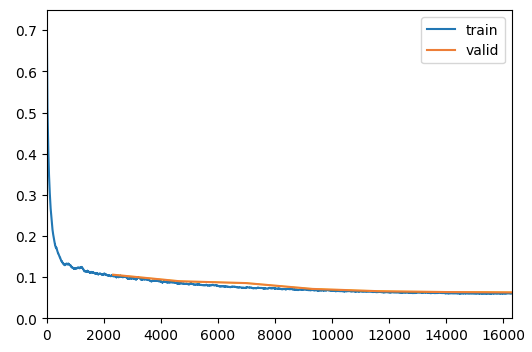
\includegraphics[width=0.7\linewidth]{imagenes/curva_xception.png}
	\caption{Curva de aprendizaje con Xception}
\end{figure}

Observamos una más rápida convergencia que \textbf{ResNet34} motivado posiblemente por los filtros de distintos tamaños. Tenemos el mismo comportamiento de bondad entre la pérdida de entrenamiento y validación. Sin embargo, obtenemos una pérdida en validación de $E_{val} \approx 0.062$ la cual es superior a la de \textbf{ResNet34} indicando que a pesar de la rápida convergencia el resultado final es mejor con un mayor número de conexiones residuales. 

A continuación observamos su reconstrucción con un resultado muy similar en apariencia.
\begin{figure}[H]
	\centering
	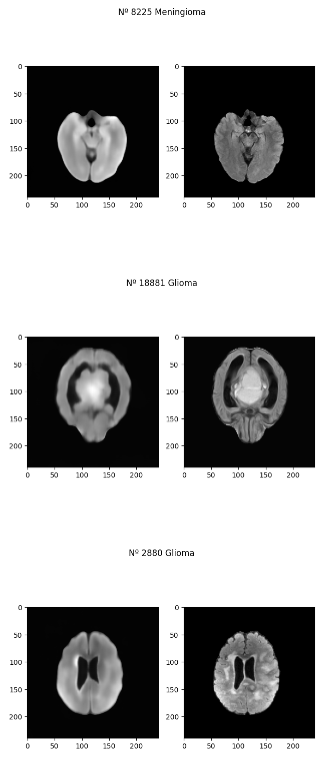
\includegraphics[width=0.4\linewidth]{imagenes/reconstruccion_xception.png}
	\caption{Reconstrucción de las imágenes con Xception}
\end{figure}

A continuación, ante los resultados de esta comparación mostramos la siguiente tabla.

\begin{table}[H]
	\centering
	\begin{tabular}{|cccccc|}
		\toprule
		Arquitectura & $E_{train}$ & $E_{val}$ \\ 
		\midrule
		\textbf{ResNet34} & \textbf{0.055986} & \textbf{0.058405} \\ 
		Xception & 0.060293 & 0.062978 \\ 
		\bottomrule
	\end{tabular}
	\caption{Pérdida de entrenamiento y validación para clasificación con la parte convolucional congelada}
	\label{tabla:resultados3}
\end{table}

Eligiendo por tanto a \textbf{ResNet34} como codificador de las arquitecturas. 

\section{Clasificación}

\subsection{Entrenamiento en clasificación}

A continuación, mostramos los experimentos realizados para la tarea de clasificación. Tomamos \textbf{ResNet34} como codificador le añadimos la representación latente y las capas densamente conectadas, entrenamos las capas fully-connected congelando las capas convolucionales (codificador y representación latente) durante $3$ épocas tomando $\approx 3$ horas con estos resultados.

\begin{table}[H]
	\centering
	\begin{tabular}{|cccccc|}
		\toprule
		epoch & train\_loss & valid\_loss & accuracy & balanced\_accuracy & time \\ 
		\midrule
		0 & 0.112794 & 0.178968 & 0.805254 & 0.781898 & 1:04:50 \\ 
		1 & 0.119699 & 0.174729 & 0.819330 & 0.773066 & 1:03:01 \\ 
		\textbf{2} & \textbf{0.083459} & \textbf{0.141255} & \textbf{0.855540} & \textbf{0.794527} & \textbf{1:04:18} \\ 
		\bottomrule
	\end{tabular}
	\caption{Pérdida de entrenamiento y validación para clasificación con la parte convolucional congelada}
	\label{tabla:resultados3}
\end{table}

\begin{figure}[H]
	\centering
	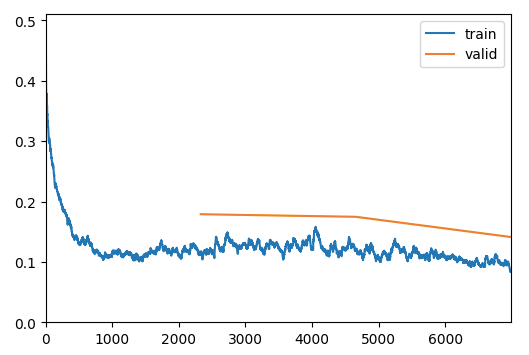
\includegraphics[width=0.7\linewidth]{imagenes/task1_freeze.png}
	\caption{Curva de aprendizaje para clasificación parte convolucional congelada}
\end{figure}

Observamos una rápida convergencia al inicio del entrenamiento, estabilizándose durante la época número $1$ y volviendo a converger ligeramente durante la época $2$. En este caso y para esta primera fase, el entrenamiento no es tan óptimo, habiendo cierta distancia entre las pérdidas de validación y entrenamiento. 

A continuación, tras estas $3$ épocas ajustando las capas densamente conectadas pasamos a descongelar toda la red para que quede mejor ajustado.

\begin{table}[H]
	\centering
	\begin{tabular}{|cccccc|}
		\toprule
		epoch & train\_loss & valid\_loss & accuracy & balanced\_accuracy & time \\
		\midrule
		0 & 0.056434 & 0.209338 & 0.855477 & 0.840139 & 1:01:57 \\ 
		\textbf{1} & \textbf{0.040761} & \textbf{0.190361} & \textbf{0.864976} & \textbf{0.812309} & \textbf{1:01:41} \\ 
		2 & 0.023256 & 0.260177 & 0.876575 & 0.832247 & 1:00:26 \\ 
		3 & 0.009723 & 0.330192 & 0.877014 & 0.834721 & 1:00:30 \\ 
		\bottomrule
	\end{tabular}
	\caption{Pérdida de entrenamiento y validación para clasificación toda la red descongelada}
	\label{tabla:resultados3}
\end{table}

\begin{figure}[H]
	\centering
	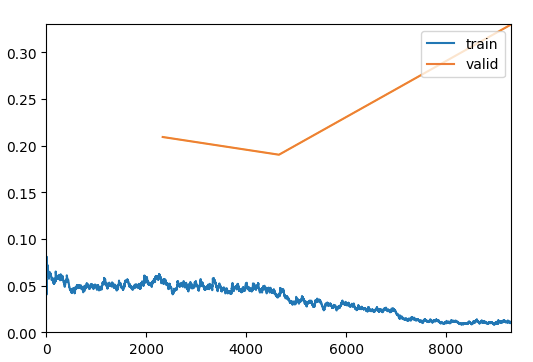
\includegraphics[width=0.7\linewidth]{imagenes/task1_unfreeze.png}
	\caption{Curva de aprendizaje para clasificación toda la red descongelada tras ajustar capas densamente conectadas}
\end{figure}

Observamos como en las dos primeras épocas tenemos convergencia en validación, tras ellos se dispara validación indicándonos que hemos llegado al resultado tope en el entrenamiento. Este proceso de entrenamiento esta configurado con \textbf{EarlyStopping} por lo que PyTorch automáticamente guarda el mejor modelo (el que haya conseguido una pérdida en validación más baja en todas las épocas) en este caso tras descongelar obtiene como modelo final el correspondiente a la época número $1$. 

Observamos como tras haber pasado el proceso de ajuste inicial de las capas densamente conectadas al descongelar todo, obtenemos unas pérdida de validación y entrenamiento mucho más dispares. Esto podría cómo las diferentes partes de la arquitectura inducen complejidad en el proceso de entrenamiento: las capas densamente conectadas (que era lo único entrenable en la primera fase) hacen que esta diferencia sea muy pequeña porque estas capas son en comparación pequeñas. Al descongelar toda las capas de la red, siendo el codificador mucho mayor que las capas densas se observa como se induce un ruido mayor.


A continuación, y a pesar de que la teoría indica que primero ajustemos las capas densamente conectadas primero congelando el resto de las capas en sus inicios, probamos a entrenar toda la red descongelada sin un ajuste previo.

\begin{table}[H]
	\centering
	\begin{tabular}{|cccccc|}
		\toprule
		epoch & train\_loss & valid\_loss & accuracy & balanced\_accuracy & time \\
		\midrule
		0 & 0.080457 & 0.178836 & 0.854348 & 0.796523 & 1:23:49 \\ 
		1 & 0.084583 & 0.175143 & 0.847827 & 0.781100 & 1:24:09 \\ 
		\textbf{2} & \textbf{0.086810} & \textbf{0.159217} & \textbf{0.852185} & \textbf{0.800501} & \textbf{1:26:20} \\ 
		3 & 0.081304 & 0.370888 & 0.832309 & 0.747997 & 1:21:31 \\ 
		\bottomrule
	\end{tabular}
	\caption{Pérdida de entrenamiento y validación para clasificación para todo el entrenamiento toda la red descongelada}
	\label{tabla:resultados6}
\end{table}


\begin{figure}[H]
	\centering
	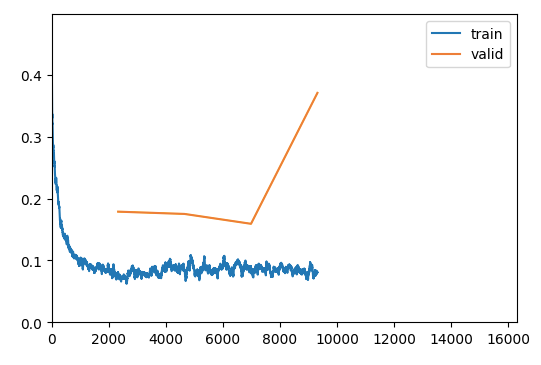
\includegraphics[width=0.7\linewidth]{imagenes/task1_totally_unfreeze.png}
	\caption{Curva de aprendizaje para clasificación todo el entrenamiento toda la red descongelada}
\end{figure}

Observamos como el mejor resultado que obtenemos es en la época número $2$ siendo peor que la mejor con la estrategia anterior. Adicionalmente, observamos como se alcanza una convergencia rápida llevando a fuerte overfitting justo en la siguiente época. Podemos interpretar como esta estrategia no sólo da peores resultados sino tiene una peor estabilidad en el proceso de entrenamiento.

\subsection{Validación en clasificación}

Tras entrenar los modelos pasamos a obtener los resultados finales infiriendo con el modelo en clasificación para los conjuntos de validación y test.

\subsubsection{Antes de aplicar votación}

En primer lugar calculamos la bondad sin aplicar el esquema de votación, la esperanza que se tiene es que tras la aplicación el esquema de votación los resultados sean iguales o mejores que los siguiente. No aplicaremos test ya que la tarea real es clasificación binaria con el esquema por lo que no es relevante el resultado de test en estas condiciones. 

A continuación, vemos los resultados obtenidos de ajuste para las métricas en entrenamiento y validación sin votación. Construimos las siguientes matrices de confusión tras la inferencia de cada conjunto.
 
\begin{figure}[H]
	\centering
	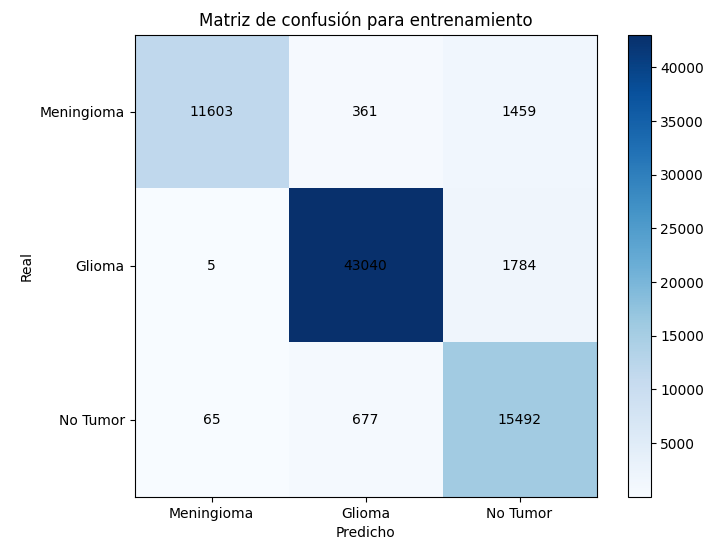
\includegraphics[width=0.7\linewidth]{imagenes/task1_results_train.png}
	\caption{Matriz de confusión de entrenamiento sin votación}
\end{figure}

\begin{figure}[H]
	\centering
	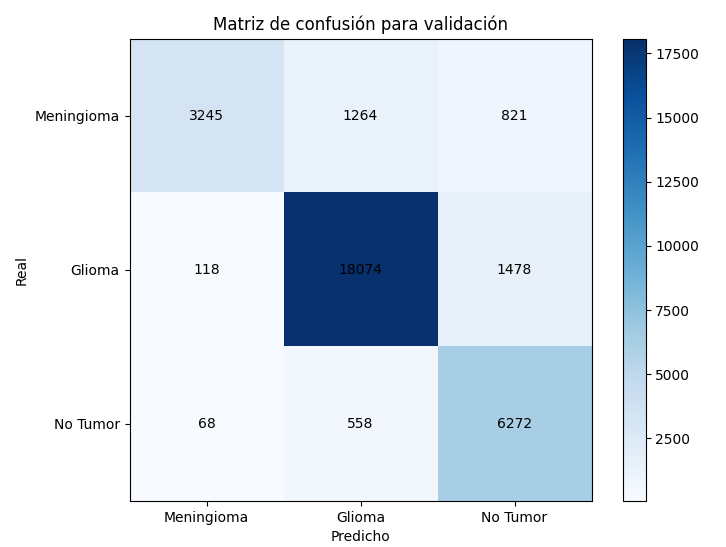
\includegraphics[width=0.7\linewidth]{imagenes/task1_results_validation.png}
	\caption{Matriz de confusión de validación sin votación}
\end{figure}

\begin{table}[H]
	\centering
	\begin{tabular}{|ccc|}
		\toprule
		Conjunto & accuracy ($\%$) & balanced\_accuracy ($\%$) \\
		\midrule
		Entrenamiento & 94.1586 & 92.6266 \\ 
		Validación & 86.4976 & 81.2309 \\ 
		\bottomrule
	\end{tabular}
	\caption{Resultados de validación y entrenamiento sin votación}
	\label{tabla:resultados10}
\end{table}

Observamos un ajuste alto en los datos de entrenamiento indicando un buen proceso de entrenamiento y resultados competitivos pero mejorables en validación. Observamos como la clase más conflictiva es \textbf{No Tumor} con las otras dos clases de tumores, indicando que la tarea más difícil es la detección del tumor y no la caracterización de este.

\subsubsection{Tras aplicar votación}

Aplicamos el esquema de votación, en primer lugar necesitamos explorar el parámetro $threshold$ que definimos en la metodología. El parámetro $threshold$ mide la tolerancia que tiene el modelo para predecir a meningioma, cuando existe un mayor número de predicciones por imagen a meningioma que $threshold$ el modelo predice toda la resonancia a meningioma, y en caso contrario a glioblastoma.

Tras hacer inferencia y ver qué cantidad promedio de predicciones de cada clase obteníamos para toda la resonancia de unos cuantos ejemplos, observamos como las predicciones a meningiomas eran muchos menores que para los gliomas. Esto está motivado por la propia naturaleza de la cantidad de imágenes de tumores de cada clase debido a que los meningiomas son más pequeños que los gliomas en promedio. 

Como definimos en la metodología necesitamos un esquema que lidie con este desbalanceo. Por ello, descartamos valores altos de $threshold$ y probamos dos valores pequeños: para $threhold = 5$ y $threshold = 3$.

A continuación mostramos las matrices de confusión asociadas a la aplicación de estos dos esquemas de votación.

\begin{figure}[H]
	\centering
	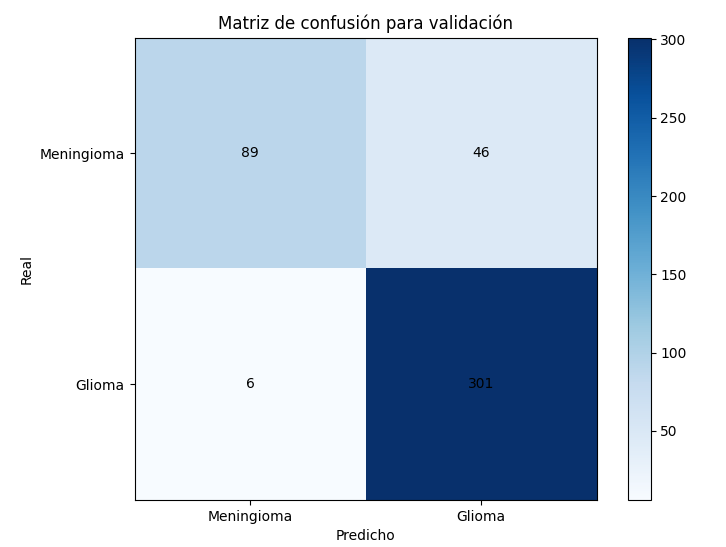
\includegraphics[width=0.7\linewidth]{imagenes/task1_val_5.png}
	\caption{Matriz de confusión de validación con votación: $Meningiomas < 5$}
\end{figure}

\begin{figure}[H]
	\centering
	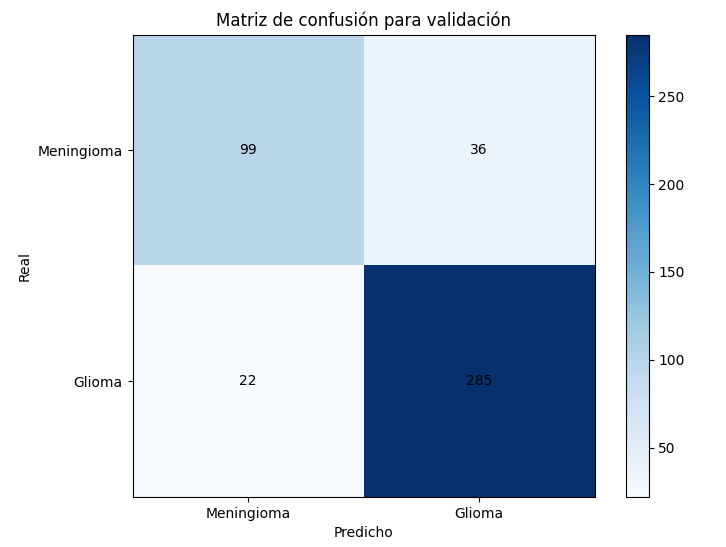
\includegraphics[width=0.7\linewidth]{imagenes/task1_val_3.png}
	\caption{Matriz de confusión de validación con votación: $Meningiomas < 3$}
\end{figure}

\begin{table}[H]
	\centering
	\begin{tabular}{|ccc|}
		\toprule
		Threshold & accuracy ($\%$) & balanced\_accuracy ($\%$) \\
		\midrule
		5 & 88.2352 & 81.9857 \\ 
		3 & 86.8779 & 83.0363  \\ 
		\bottomrule
	\end{tabular}
	\caption{Resultados de validación con votación y de la búsqueda}
	\label{tabla:resultados11}
\end{table}

Observamos como obtenemos un mejor accuracy balanceado con $threshold = 3$, así que optamos por su elección.
Tras haber configurado $threshold = 3$ y haber visto su bondad en validación solo queda obtener el resultado final con test.

\begin{figure}[H]
	\centering
	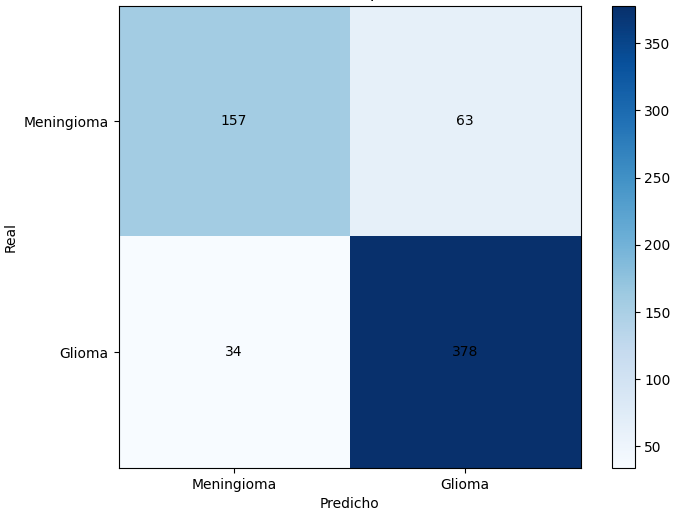
\includegraphics[width=0.8\linewidth]{imagenes/task1_test.png}
	\caption{Matriz de confusión de Test con votación}
\end{figure}

Obtenemos resultados finales para test, obteniendo un accuracy del $84.6519 \%$ y un accuracy balanceado del $81.5556 \%$. Con este resultado sabemos que la obtención de un modelo final debería tener un accuracy balanceado en clasificación $ Acc_{F} \geq 81.5556 \% $.

\subsection{Comparativa de clasificación con el estado del arte}

Para finalizar la experimentación de esta primera tarea ponemos en contexto estos resultados con el estado del arte. Aunque no sean del todo comparables debido no son formulaciones del problema idénticas (se tiene otro tipo de tumor en el estado del arte) y se utilizan conjuntos de datos distintos T1-CE image en el estado del arte frente a BraTS en el este trabajo. Sin embargo, es importante hacer una observación de la bondad de los resultados teniendo en cuenta estas diferencias. 

\begin{table}[H]
	\centering
	\begin{tabular}{|cccc|}
		\toprule
		Autor & accuracy ($\%$) & balanced\_accuracy ($\%$) & $P_{test}$ \\
		\midrule
		\cite{cheng2015enhanced} & 91.2 & - & 61\\ 
		\cite{cheng2016retrieval} & 94.7 & - & 61\\ 
		\cite{abiwinanda2019brain} & 84.1 & - & 70\\ 
		\cite{pashaei2018brain} & 81.0 & - & 70\\ 
		\cite{sultan2019multi} & 96.1 & - & 75\\
		\cite{diaz2021deep} & 97.3 & - & 46 \\  
		Nuestro método & 84.65 & 81.56 & 632 \\ 
		\bottomrule
	\end{tabular}
	\caption{Resultados de validación con votación y de la búsqueda}
	\label{tabla:resultados12}
\end{table}

Los resultados del estado del arte no incluyen un validación con un esquema balanceado lo cual lo hace soluciones mucho menos generales y reales. Añadimos a la tabla, la entrada $P_{test}$ que la cantidad de pacientes que se usaron en el conjunto de test de cada trabajo.

Nuestro trabajo está validado en un conjunto de test $\approx 8$ veces mayor que el mayor conjunto utilizado en la literatura y utiliza una política de aprendizaje balanceado lo cual puede hacer obtener peores resultados en un métrica más débil como puede ser accuracy sin balanceo. Aún así nuestro método supera a 2 de los 6 métodos presentados en la revisión histórica.

\section{Segmentación}

En esta sección recogemos los experimentos y resultados de estos para la tarea de segmentación. 

\subsection{Entrenamiento en segmentación}
Entrenamos la arquitectura enteramente descongelada con tamaño de lote de $32$ ejemplos durante $7$ épocas alcanzando el entrenamiento una duración de $ \approx 8$ horas. A continuación se presenta la tabla y curva de aprendizaje obtenidas.
\begin{table}[H]
	\centering
	\begin{tabular}{|ccccc|}
		\toprule
		epoch & train\_loss & valid\_loss & Dice Loss & time \\ 
		\midrule
		0 & 0.095941 & 0.319656 & 0.319656 & 1:34:08 \\ 
		\textbf{1} & \textbf{0.073242} & \textbf{0.258797} & \textbf{0.258797} & \textbf{1:32:56} \\ 
		2 & 0.059904 & 0.284256 & 0.284256 & 1:34:48 \\ 
		3 & 0.050076 & 0.274452 & 0.274452 & 1:37:00 \\ 
		4 & 0.046783 & 0.266702 & 0.266702 & 1:40:18 \\ 
		\bottomrule
	\end{tabular}
	\caption{Pérdida de entrenamiento y validación para segmentación toda la red descongelada}
	\label{tabla:resultados4}
\end{table}

\begin{figure}[H]
	\centering
	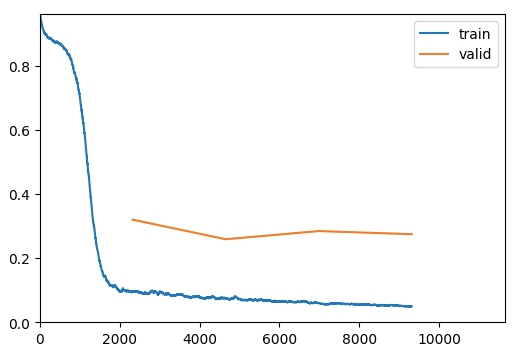
\includegraphics[width=0.7\linewidth]{imagenes/curva_segmentation.png}
	\caption{Curva de aprendizaje para la tarea de segmentación}
\end{figure}

Observamos como tenemos una muy rápida convergencia en la primera época y cómo se estabiliza en las sucesivas épocas refinándose la pérdida Dice muy ligeramente. En este tiempo de cómputo limitado observamos como no se produce overfitting. Sin embargo, obtenemos un error de validación que disminuye muy poco entre la primera y segunda época aumentando ligeramente en las sucesivas épocas. Podemos interpretar que existe un comportamiento estable en todo el proceso de entrenamiento.

A continuación, comparamos la salida del modelo respecto la imagen real. Esta salida es previa a aplicarle un proceso de umbralización con la cual obtendríamos una máscara binaria final. El proceso de umbralización que se aplicará consiste en determinar como píxeles segmentados (usando la etiqueta 1) los píxeles cuyo valor sea mayor a un umbral $U$ y en caso contrario, píxeles no segmentados (usando la etiqueta 0). El umbral $U$ empleado será $U = 0.8$. Viendo en la práctica como este umbral o uno ligeramente más bajo como $0.5$ no afecta significativamente a los resultados. 
\begin{figure}[H]
	\centering
	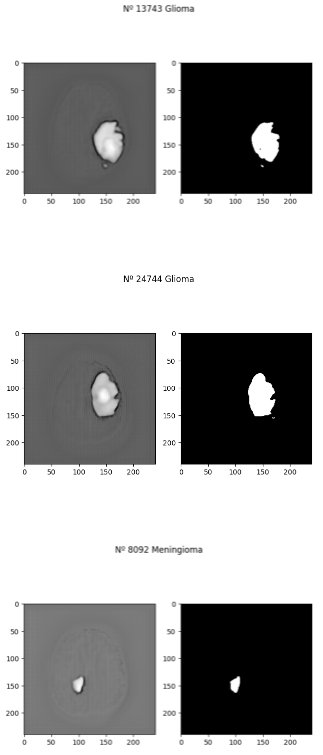
\includegraphics[width=0.5\linewidth]{imagenes/output_segmentation.png}
	\caption{Comparación de la salida del modelo respecto la real}
\end{figure}
Observamos buenos resultados consiguiendo máscaras de segmentación que replican en detalle la segmentación original. En la imagen producida por la red se puede apreciar la sombra de un cerebro pudiendo ver un efecto residual del codificador y del uso de skip connections.

\subsection{Validación en segmentación}

A continuación, inferimos los resultados finales para segmentación en validación y test para nuestras tres métricas. Recogemos en la siguiente tabla estos resultados.

\begin{table}[H]
	\centering
	\begin{tabular}{|cccc|}
		\toprule
		Partición & Similaridad Dice & Distancia Hausdorff & Sensibilidad \\ 
		\midrule
		Validación & 0.777343 & 14.573561 & 0.720415 \\ 
		Test & 0.772642 & 14.577154 & 0.709075 \\ 
		\bottomrule
	\end{tabular}
	\caption{Resultados de hold-out en validación y test para segmentación}
	\label{tabla:resultados5}
\end{table}
Observamos que ambos conjuntos mantienen resultados muy similares empeorando ligeramente en test indicando robustez y coherencia en los resultados. Observamos que la peor métrica obtenida es la distancia Hausdorff que es demasiado alta, indicando que existe una distancia máxima media de $\approx 14$ píxeles entre la segmentación original y la salida del modelo. Podría significar un problema de creación de artefactos por parte del modelo.

A continuación, para darle explicabilidad a los resultados se muestra el histograma de los resultados de las métricas para todos los ejemplos, primero del conjunto de validación y después para el conjunto de test. De esta forma, podríamos identificar ejemplos especialmente difíciles y caracterizarlos.
\begin{figure}[H]
	\centering
	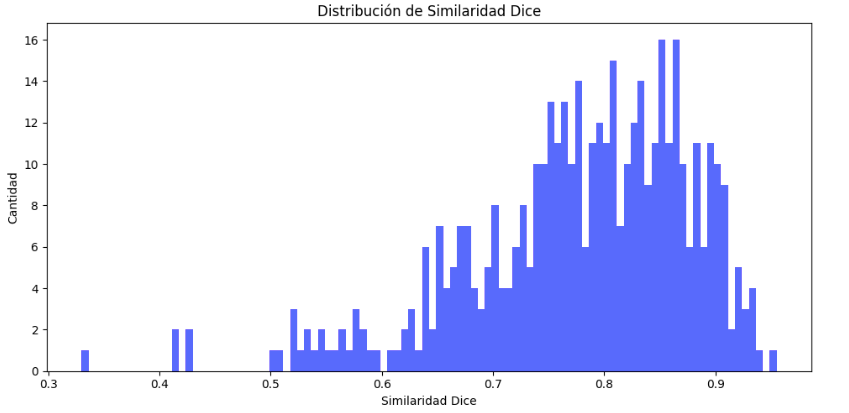
\includegraphics[width=0.7\linewidth]{imagenes/dist_dice_val.png}
	\caption{Distribución de similaridad Dice en el conjunto de validación}
\end{figure}

\begin{figure}[H]
	\centering
	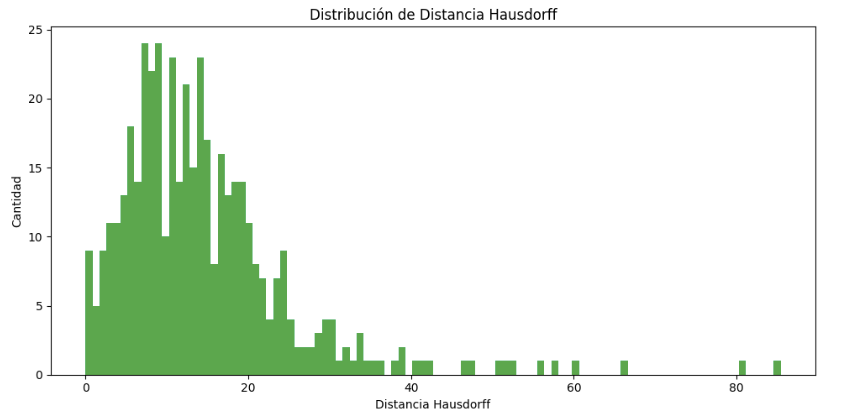
\includegraphics[width=0.7\linewidth]{imagenes/dist_haus_val.png}
	\caption{Distribución de distancia Hausdorff en el conjunto de validación}
\end{figure}

\begin{figure}[H]
	\centering
	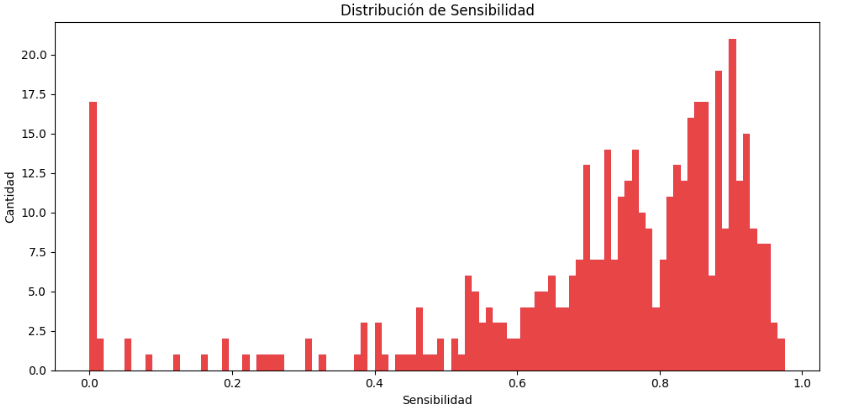
\includegraphics[width=0.7\linewidth]{imagenes/dist_sen_val.png}
	\caption{Distribución de sensibilidad en el conjunto de validación}
\end{figure}

\begin{figure}[H]
	\centering
	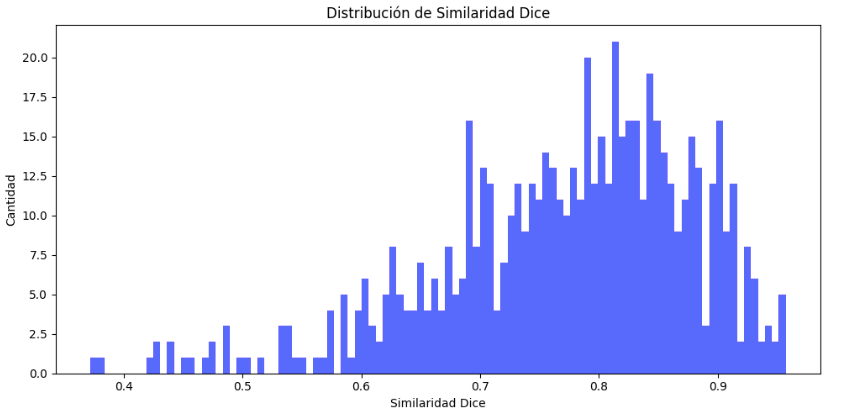
\includegraphics[width=0.7\linewidth]{imagenes/dist_dice_test.png}
	\caption{Distribución de similaridad Dice en el conjunto de test}
\end{figure}

\begin{figure}[H]
	\centering
	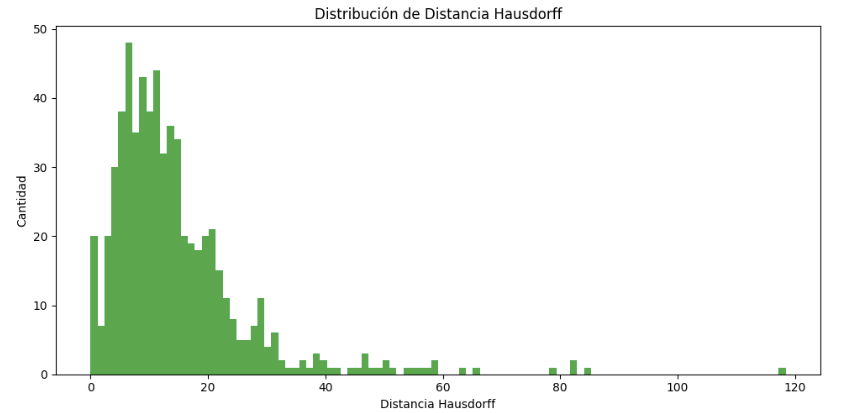
\includegraphics[width=0.7\linewidth]{imagenes/dist_haus_test.png}
	\caption{Distribución de distancia Hausdorff en el conjunto de test}
\end{figure}

\begin{figure}[H]
	\centering
	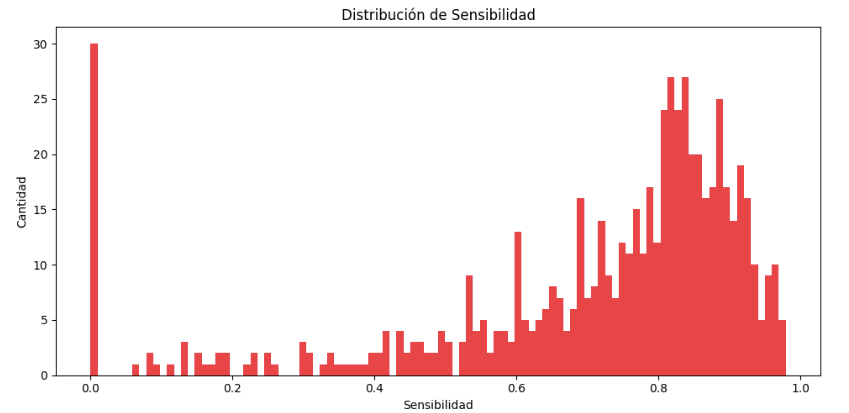
\includegraphics[width=0.7\linewidth]{imagenes/dist_sen_test.png}
	\caption{Distribución de sensibilidad en el conjunto de test}
\end{figure}

Los histogramas de estas métricas revelan una distribución en forma de campana de Gauss, lo cual es indicativo de una distribución normal. Este patrón indica robustez dentro del modelo de segmentación, observando que no existe un subconjunto de ejemplos que no puede segmentar bien. Nos sirve como prueba para demostrar la generalidad del modelo conseguida a pesar de poder obtener un modelo mejor.

La normalidad de las distribuciones también implica que las métricas son simétricas y centradas alrededor de un valor promedio consistente, lo que es indicativo de un rendimiento estable.

\subsection{Comparativa de segmentación con el estado del arte}

Para finalizar la experimentación de esta segunda tarea ponemos en contexto estos resultados con el estado del arte. Todos estos resultados han sido evaluados por conjuntos de mismo dataset \textbf{BraTS}, y respetando la misma proporción entre entrenamiento-test que la seguida en este trabajo.

En la siguiente tabla se muestran las métricas y un apartado de recursos que indica la GPU que usaron para el entrenamiento. En nuestro método usamos una gráfica Tesla P100 limitados semanalmente $30$ horas y en cada ejecución a $12$ horas. Por lo que, no podemos entrenar más de $12$ horas seguidas.

\begin{table}[H]
	\centering
	\begin{tabular}{|ccccc|}
		\toprule
		Autor & Dice ($\%$) & Hausdorff & Recall ($\%$) & Recursos \\
		\midrule
		\cite{chen2021transunet} & 78.73 & 5.0 & - & 8 x Tesla V100 \\
		\cite{zhou2021latent} & 87.1 & 6.5 & 86.8 & Quadro P5000 \\
		\cite{myronenko20193d} & 90.4 & 4.4 & - & 8 x Tesla V100\\   
		\cite{hatamizadeh2021swin} & 92.6 & 5.8 & - & 8 x Tesla V100 \\ 
		\cite{ferreira2024we} & 92.9 & 4.26 & - & 6 x RTX 6000\\
		Nuestro método & 77.3 & 14.5 & 70.9 & Tesla P100 \\ 
		\bottomrule
	\end{tabular}
	\caption{Comparativa de segmentación con el estado del arte}
	\label{tabla:resultados13}
\end{table}

Como vemos nuestro método es peor que todo el estado del arte reciente que sea comparable. Sin embargo, es una buena aproximación para las capacidades de recursos en términos de capacidad (memoria del dispositivo GPU) y rendimiento de GPU que teníamos frente las del resto de autores que son inmensamente mayores. 
